\chapter{Formation of Rainbow}

\section*{Objectives}

\begin{enumerate}
\item To study the refraction, internal reflection and dispersion of light due to a water drop which gives rise to a rainbow.
\item To study the second order rainbows formed due to drops of different liquids. 
\item To determine the refractive index of an unknown liquid A.
\end{enumerate}

\section*{Apparatus}

\begin{enumerate}
\item A modified spectrometer 
\item An incandescent lamp
\item A power supply for the lamp
\item A holder for the syringe 
\item Four small syringes 
\item Four small beakers 
\item Four small Petri dishes 
\item A magnifying reading torch 
\item Water, glycerine, clove oil, and an unknown liquid A (5 ml each)
\item A spirit level 
\item Light blocking screen
\end{enumerate}

\section*{Introduction}
The rainbow is probably one of the most spectacular light shows observed naturally in the sky. The conventional explanation to the formation of a rainbow is that sunlight -- which is composed of a spectrum of colours -- is separated into its constituent colours by the large number of water droplets present in the air on a rainy day, very much like the dispersion of light by a prism. 

However, as we shall see, this is not the full story. To completely understand the formation of the rainbow and its location in the sky, we need to take into account the fact that the droplets are actually spherical, and that incident light may be reflected internally many times before exiting the drop.

In the case of a primary (or first order) rainbow, the sunlight incident on a raindrop is refracted at the front surface, internally reflected at the back surface and refracted again as it emerges into the air as shown in Figure (\ref{fig:firstorder}). 

\begin{figure}[!htb]
    \centering
    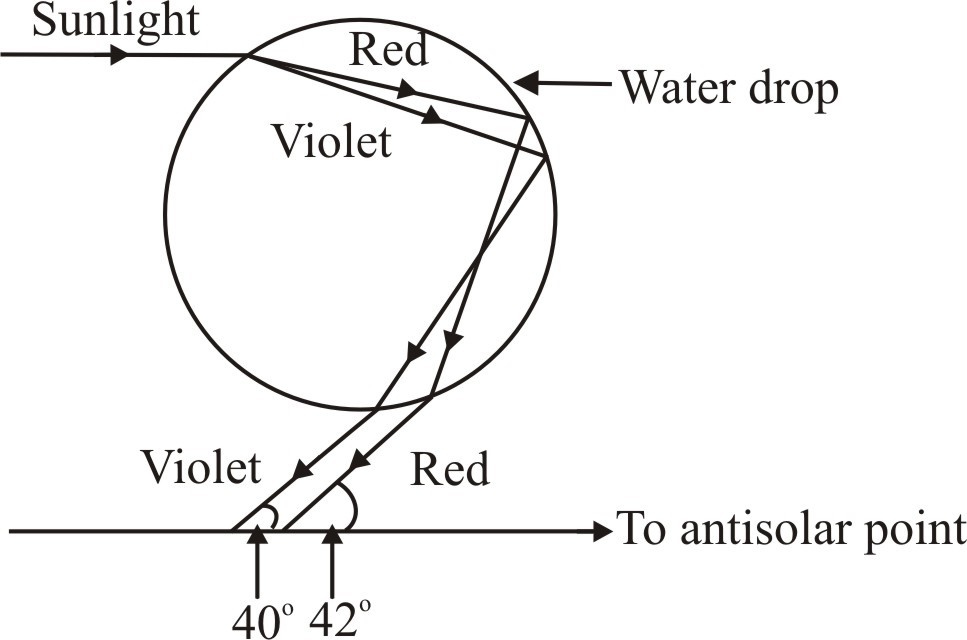
\includegraphics[width=0.5\textwidth]{figs/img1.jpg}
    \caption{Ray diagram for the formation of a primary (first order) rainbow}
    \label{fig:firstorder}
\end{figure}


However, it is possible for sunlight to be reflected internally twice, before exiting the drop. While the intensities of such light rays will be much weaker than those that have been reflected only once, it is possible to see such `secondary' (or second-order) rainbows in nature. Secondary rainbows -- as we shall see -- are formed at angles that are further out from their primary counterparts. Thus, we speak of the `order' of a rainbow as the number of times light has been totally internally reflected within the drop. Higher order rainbows are almost never seen naturally, as they are weaker than the background brightness of the sky and are usually positioned inconveniently with respect to the sun; if you are lucky, you can sometimes see a second-order rainbow. 

An instructive way to understand the formation of rainbows is to actually study the dispersion of white light by a spherical drop of water, as we shall in the present problem. (Note, however, that we use the word `rainbow' very loosely, to mean a `rainbow like \textit{spectrum}' rather than the more familiar `rainbow' in the sky.) 



\section*{Description}
In \textbf{Part A}, you will study the formation of rainbows of different orders by a suspended drop of water and measure their angular positions. You can observe these rainbows directly with your eye and can measure their angular positions using a telescope and a circular scale. For this, you will need to study the variation with respect to order of the total deviation of the incident light.

In \textbf{Part B}, you will obtain the rainbows with different liquids and measure the total deviation for the second order rainbow for different liquids.

In \textbf{Part C \textit{(optional)}}, you will use this data to determine the refractive index of the unknown liquid A. 


\section*{Theory}

We will be dealing with the propagation of light between different transparent materials. When light moves from one medium to another, it changes direction through a process known as \textit{refraction}. Thus, at least for the purposes of this experiment, we can characterise different transparent media by their refractive indices: a dimensionless number ($\mu$) which describes how much light bends when it enters the medium from vacuum. 

\begin{figure}[!htb]
\captionsetup[subfigure]{justification=centering}
\centering
        \begin{subfigure}[b]{0.5\textwidth}
        \centering
                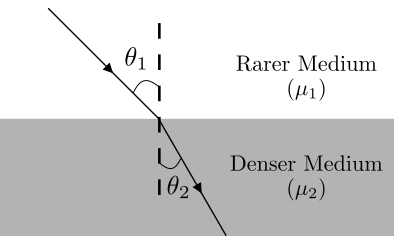
\includegraphics[scale=0.5]{figs/snell1.png}
                \caption{$\mu_1<\mu_2:$\\ The refracted ray is deviated towards normal.}
                \label{fig:rareToDense}
        \end{subfigure}\hfill
        \begin{subfigure}[b]{0.5\textwidth}
        \centering
                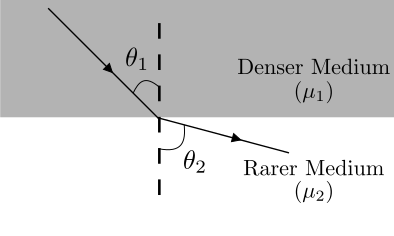
\includegraphics[scale=0.5]{figs/snell2.png}
                \caption{$\mu_1>\mu_2:$\\ The refracted ray is deviated away from normal.}
                \label{fig:denseToRare}
        \end{subfigure}
        \par\bigskip
        \begin{subfigure}[b]{\textwidth}
        \centering
                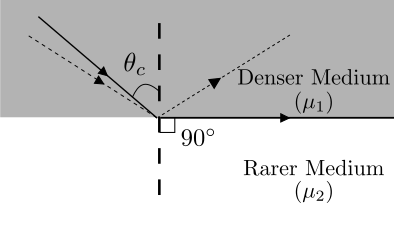
\includegraphics[scale=0.5]{figs/snell3.png}
                \caption{$\mu_1>\mu_2:$\\ Beyond some $\theta_c$, the refracted ray is reflected internally.}
                \label{fig:til}
        \end{subfigure}
        \caption{The propagation of a ray of light between media of different refractive indices.}\label{fig:snells}
\end{figure}


The relationships between the angles $\theta_1$ and $\theta_2$ (shown in Figure (\ref{fig:snells})) is given by the Sahl-Snell–Descartes law (usually called Snell's law):

 \begin{equation}
    \mu_1 \sin{\theta_1}= \mu_2 \sin{\theta_2}.
    \label{snell}
 \end{equation}

As light passes from a rarer to a denser medium (as shown in Figure (\ref{fig:rareToDense})), the ray of light bends \textit{towards} the normal, while as light travels from a denser to a rarer medium (Figure (\ref{fig:denseToRare})), the ray of light bends \textit{away} from the normal. When light moves from a denser to a rarer medium ($\mu_1>\mu_2>1$), there must be \textit{some} angle (let's call it $\theta_c$) greater than which the resulting refracted ray bends back inwards (Figure (\ref{fig:til})). This phenomenon, called \textbf{Total Internal Reflection}, plays a crucial role in the formation of the rainbow.



\subsection*{The Primary Rainbow}

Consider Figure (\ref{fig:firstorder1}) for first order $(K = 1)$ rainbow formed by a spherical drop of liquid with refractive index $\mu$.

\begin{figure}[!htb]
    \centering
    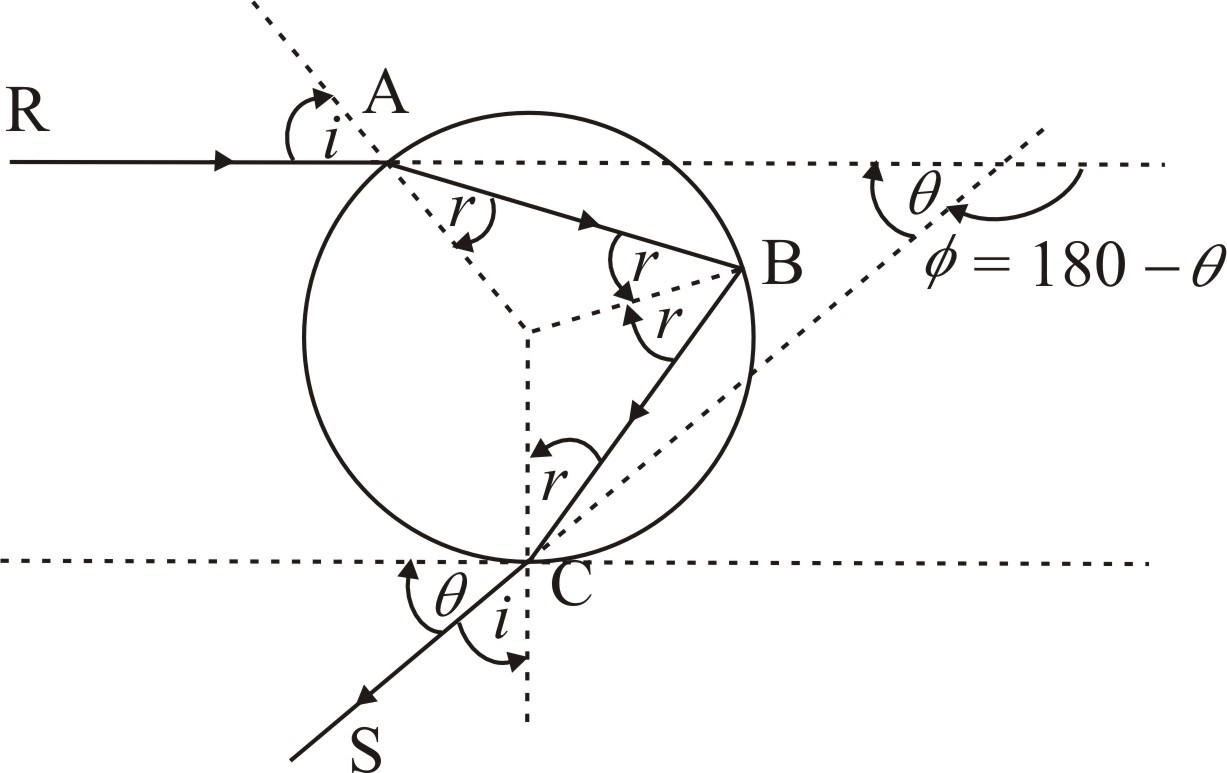
\includegraphics[width=0.5\textwidth]{figs/img3.jpg}
    \caption{Ray diagram for the formation of a first order rainbow, with angles marked.}
    \label{fig:firstorder1}
\end{figure}


Let $RABCS$ be the path of a ray of incident monochromatic light, which comes out of a spherical droplet of liquid after suffering two refractions at $A$ and $C$ and one reflection at $B$.

Let $i$ be the angle of incidence and $r$ be the angle of refraction at $A$. It should be clear to you that $r$ is also the angle of incidence and reflection at $B$. At the point $C$, since the angle of incidence inside the droplet is $r$, the angle of emergence (at $C$) will be $i$. We can then say that the \textit{deviation} of the ray due to refraction at both $A$ and $C$ is $(i-r)$. The deviation of ray due to reflection at $B$ is $(180 - 2r)$. Thus the total deviation is

\begin{equation}
\phi_{1}=2(i-r)+(180-2r)
\end{equation}


\begin{figure}[!htb]
    \centering
    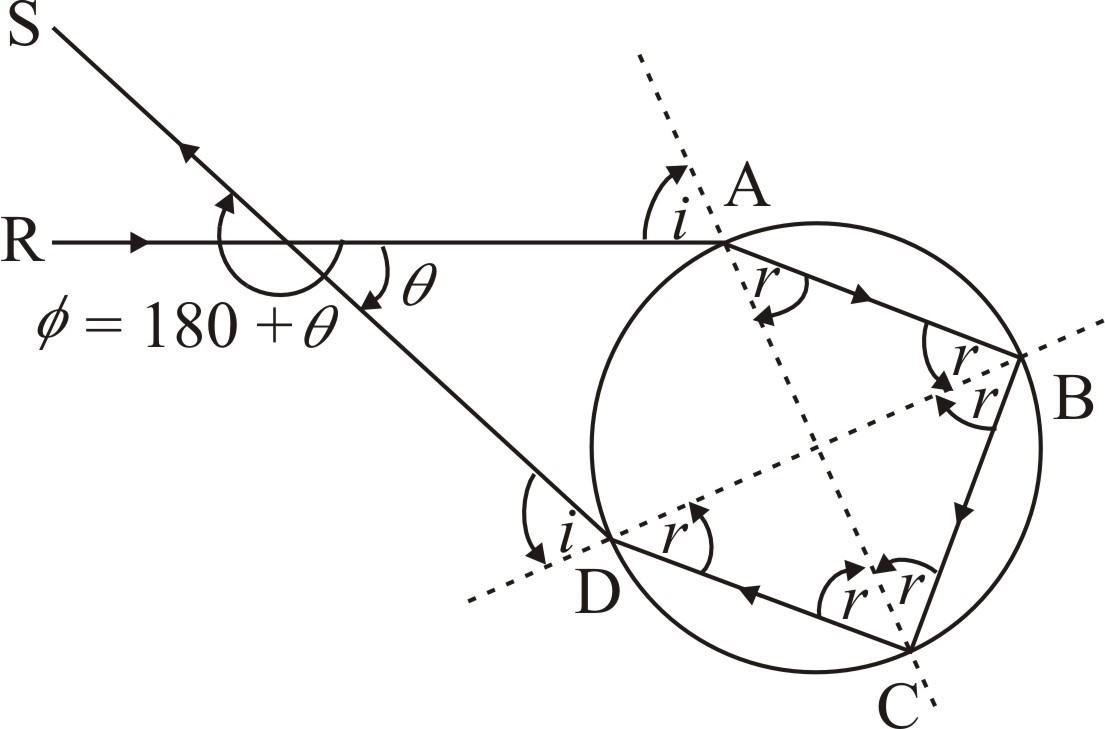
\includegraphics[width=0.5\textwidth]{figs/img4.jpg}
    \caption{Ray diagram for the formation of a second order rainbow, with angles marked.}
    \label{fig:secondorder}
\end{figure}


If we now consider the second order rainbow, there will be two internal reflections as shown in Figure (\ref{fig:secondorder}). The deviations due to each of the reflections will be the same, and thus the total deviation due to reflections is $2\times (180 - 2r)$. Similarly for $K^\text{th}$ order rainbow (corresponding to $K$ internal reflections) the deviation is $K\times(180 - 2r)$. As there are only two refractions (one at the point of incidence, and one at the point of emergence), the total deviation $\phi_K$ suffered by the emergent ray after $K$ internal reflections will be

\begin{equation*}
    \phi_K = 2(i-r) + K(180-2r)
\end{equation*}

or more simply, 

\begin{equation}
    \phi_K = 180K + 2i - 2r(K+1)
    \label{mindevK}
\end{equation}


\subsubsection*{The angle of minimum deviation}

The rays that make up the rainbow were reflected at least once inside the drop, but not all the reflected rays contribute; the rest emerge at different angles and are not visible to the observer. The main reason higher-order rainbows are not visible in the sky is the glare of sunlight directly transmitted or reflected from raindrops. In our experiment too this `glare' tends to obscure the rainbows, but it is more easily controlled. Since only the light falling on a part of the drop contributes to a given rainbow, and the bright glare spots often result from light striking another part, it is therefore possible reduce the glare by masking a part of the incident beam.

Let us thus imagine that only half the drop is illuminated (as will be done in this experiment): all the parallel rays are refracted when they enter the drop, and then reflected by the interior surface before being refracted as they leave. It should be clear (as can be seen in Figure (\ref{fig:rainbowDeviation})) that the emerging light is scattered over a large range of angles, depending on where the deviating ray makes contact with the drop's surface. At a certain position in the drop, a \textbf{minimum deviation point} is reached. Rays that strike the drop around this point are `bunched' together, and their brightness is further enhanced. It is precisely this phenomenon that makes the rainbow more visible in the sky than other scattered light. 


\begin{figure}[!htb]
    \centering
    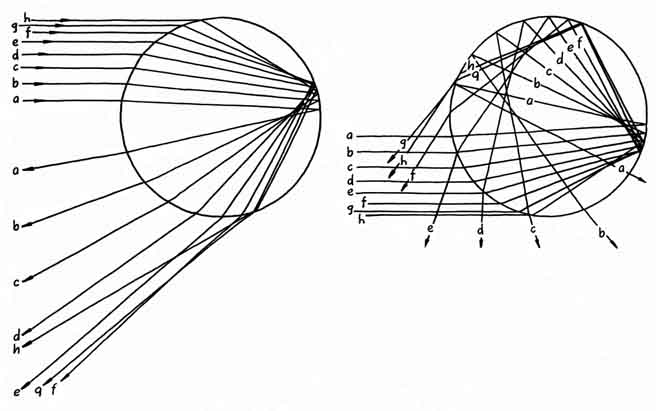
\includegraphics[width=0.75\textwidth]{figs/rainbowDeviation.jpeg}
    \caption{Ray paths forming a primary rainbow (\textit{left}) and a secondary rainbow (\textit{right}): The rays $f$ and $g$ in the primary rainbow and $g$ and $h$ in the secondary rainbow are `bunched' together as they are close to the angle of minimum deviation. \texttt{Source:[1]}}
    \label{fig:rainbowDeviation}
\end{figure}



We will thus observe the rainbow at the minimum value of $\phi_K$, which we can find by enforcing the condition\footnote{That this condition represents the case of minimum deviation is clear from the fact that if $\frac{\dd^2 \phi_K}{\dd i^2}$ is calculated, it is found to be positive.}  $$\frac{\dd\phi_K}{\dd i}=0.$$

\begin{imp}
The index of refraction -- which determines how much the rays are being bent on entering or leaving the drop -- is different for each colour,\footnote{You will understand why this is the case in a later course on optics.} and as a result, each colour has a different angle of minimum deviation, where the scattered light is most intense. The first-order rainbow can thus be found between 137.6 degrees (for red) and 139.4 degrees (for blue).
\end{imp}

\begin{figure}[!htb]
    \centering
    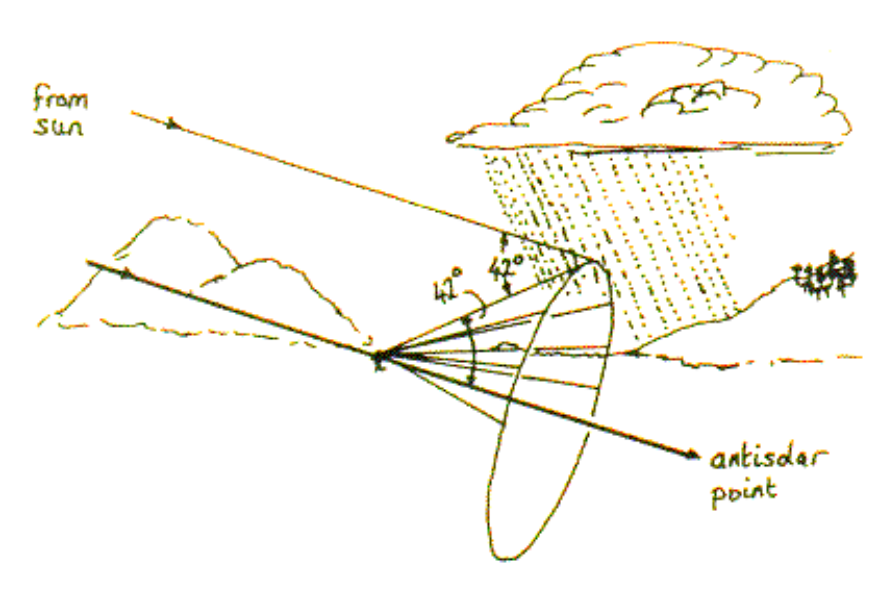
\includegraphics[width=0.5\textwidth]{figs/rainarc.png}
    \caption{Angular position of the primary rainbow in the sky.}
    \label{fig:rainbowSky}
\end{figure}


\begin{question}
\paragraph{Question:} Suppose for a moment that the refractive index of materials \textbf{didn't} depend on the wavelength of light. In this case, rainbows would:
\begin{enumerate}
\itemsep0em
    \item Remain unchanged.
    \item Not be formed.
    \item Simply be a bright white band of light.
\end{enumerate}

\paragraph{Question:} Can you now explain where the $42^\circ$ comes from in Figure (\ref{fig:rainbowSky})?
\end{question}

Differentiating Equation (\ref{mindevK}), we have

\begin{equation*}
\begin{aligned}
\frac{\dd\phi_{K}}{\dd i}&=2-2\frac{\dd r}{\dd i}-2K\frac{\dd r}{\dd i}\\
&=2-2(K+1)\frac{\dd r}{\dd i}\\
\frac{\dd \phi_{K}}{\dd i}&=0\Rightarrow2-2(K+1)\frac{\dd r}{\dd i}=0
\end{aligned}
\end{equation*}

Hence,         
\begin{equation}
    \frac{\dd r}{\dd i}=\frac{1}{K+1}
    \label{mindevcond}
\end{equation}

Thus, for a $K^\text{th}$ order rainbow at the angle of minimum deviation, Equation (\ref{mindevcond}) relates the angle of refraction to the angle of incidence. However, we also know that the angle of refraction and angle of incidence are related by the refractive index of the drop through Equation (\ref{snell}). For a drop of refractive index $\mu$, we can rewrite it as:\footnote{The refractive index of air can be taken to be $1$.}

\begin{equation}
    \mu = \frac{\sin{i}}{\sin{r}}
    \label{snellir}
\end{equation}

 or equivalently,
 
 \begin{equation}
     r = \sin^{-1}\left(\frac{\sin{i}}{\mu}\right).
     \label{rasfnofu}
 \end{equation}

We can use  Equations (\ref{rasfnofu}) and (\ref{mindevK}) to relate the total deviation $\phi_K$ for the $K^\text{th}$ order rainbow to the angle of incidence $i$ and the refractive index $\mu$:
 
 \begin{equation}
     \phi_K = 180K + 2i - 2(K+1)\sin^{-1}\left(\frac{\sin i}{\mu}\right)
     \label{phiKi}
 \end{equation}

In particular, for $K = 2$, one can show -- using Equations (\ref{phiKi}) and (\ref{iK}) -- that 

\begin{equation}
   \cos\left( \frac{\phi_2}{6}\right) = \frac{1}{\mu}\left( 3 \cos\left(\frac{i + 180}{3}\right) \cos{i} + \sin\left(\frac{i + 180}{3}\right)\sin{i} \right)
\end{equation}


We could also derive a relation between the angle of incidence and the refractive index for different orders of rainbows. Differentiating Equation (\ref{snellir}) with respect to $i$, we obtain,
 \begin{equation*}
     \cos i = \mu\cos r \frac{\dd r}{\dd i}
\end{equation*}

Substituting the expression for $\frac{\dd r}{\dd i}$ from Equation (\ref{mindevcond}) in the above equation, and using the Snell's law relation and the trigonometric identity, $\sin^2 x + \cos^2 x = 1$, we have
\begin{equation}
\cos i=\frac{\sqrt{\mu^{2}-\sin^{2}i}}{K+1}
\end{equation}
Squaring both sides, and using the same trigonometric identity again, the equation $(K^2 + 2K)\cos^2 i = (\mu^2 - 1)$ is obtained.
Hence, we have
\begin{equation}
    \cos i = \sqrt{\frac{\mu^2 - 1}{K(K+2)}}.
    \label{iK}
\end{equation}
 
 
\begin{figure}[!htb]
    \centering
    \begin{subfigure}[b]{0.5\linewidth}
    \centering
    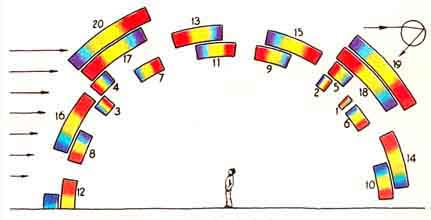
\includegraphics[width=\textwidth]{figs/multipleRainbows.jpeg}
    \end{subfigure}%
    \begin{subfigure}[b]{0.5\linewidth}
    \centering
    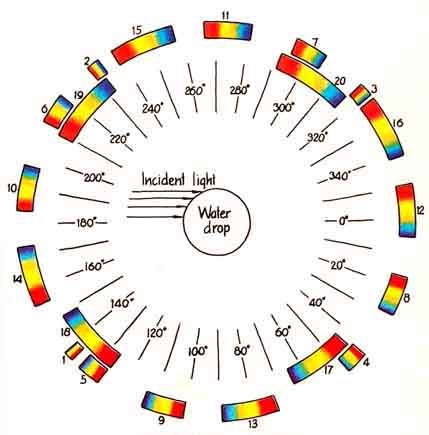
\includegraphics[width=0.75\textwidth]{figs/multipleRainbowsLab.jpeg}
    \end{subfigure}
    \caption{Rainbows represented as they would appear in the sky (\textit{left}) and in this experiment (\textit{right}), relative to the incident beam of light. \texttt{Source:[1]}}
    \label{fig:rainbow}
\end{figure}

 
\section*{Experimental Setup}

\subsection*{The (modified) spectrometer}

A spectrometer is an optical instrument, which may be used to study the spectrum, dispersion, refraction, reflection etc. It can be used to measure the angles. It consists of four parts: a collimator, a telescope, a prism table and a circular scale disc.

The \textbf{collimator} is used to obtain a parallel beam of light. The collimator is a tube with a lens at the back (called the collimator lens) and an adjustable slit at the front. The distance between the slit and the collimator lens can be adjusted with the help of a knob fixed to its body. The \textbf{telescope} is used to collect and observe parallel light. The telescope is another tube with an arrangement of lenses (called the objective and the eyepiece) at the ends. The distance between the objective and the eyepiece may also be adjusted. The \textbf{prism table} is a circular table with levelling screws, which is mounted at the centre of the circular scale disc. The prism table is used to mount optical components (prisms, obviously, but also gratings, etc.).  The \textbf{circular scale disc} is used to measure and record the position of the telescope arm and thus measures the angle of displacement. The circular scale disc has three scales, a circular main scale and two identical vernier scales. The vernier scales are fixed along two windows to the prism table and the circular main scale moves with telescope arm.  

\textbf{Modifications:} In the modified spectrometer, the mounting base of the collimator arm has been extended to move the collimator away from the circular base and hence increase the range of movement of the telescope. The collimator is provided with an extra adjustable slit mounted externally on its back. This extra slit allows us to block the light falling on one side of the liquid drop so that only one half of the liquid drop is illuminated. The telescope does not have the regular lens arrangement, but instead the eyepiece is replaced by a pinhole and the objective is replaced by a lens of suitable focal length. This is done to obtain a magnified image of the drop. The circular scale disc is kept as it is. 

A specially designed holder is fixed on the prism table, within which a syringe may be clamped. The holder is designed so that when the syringe is clamped properly and the drop is obtained, the drop is seen from all the angular positions of the telescope exactly at the centre of field of view. 

\begin{figure}[!htb]
    \centering
    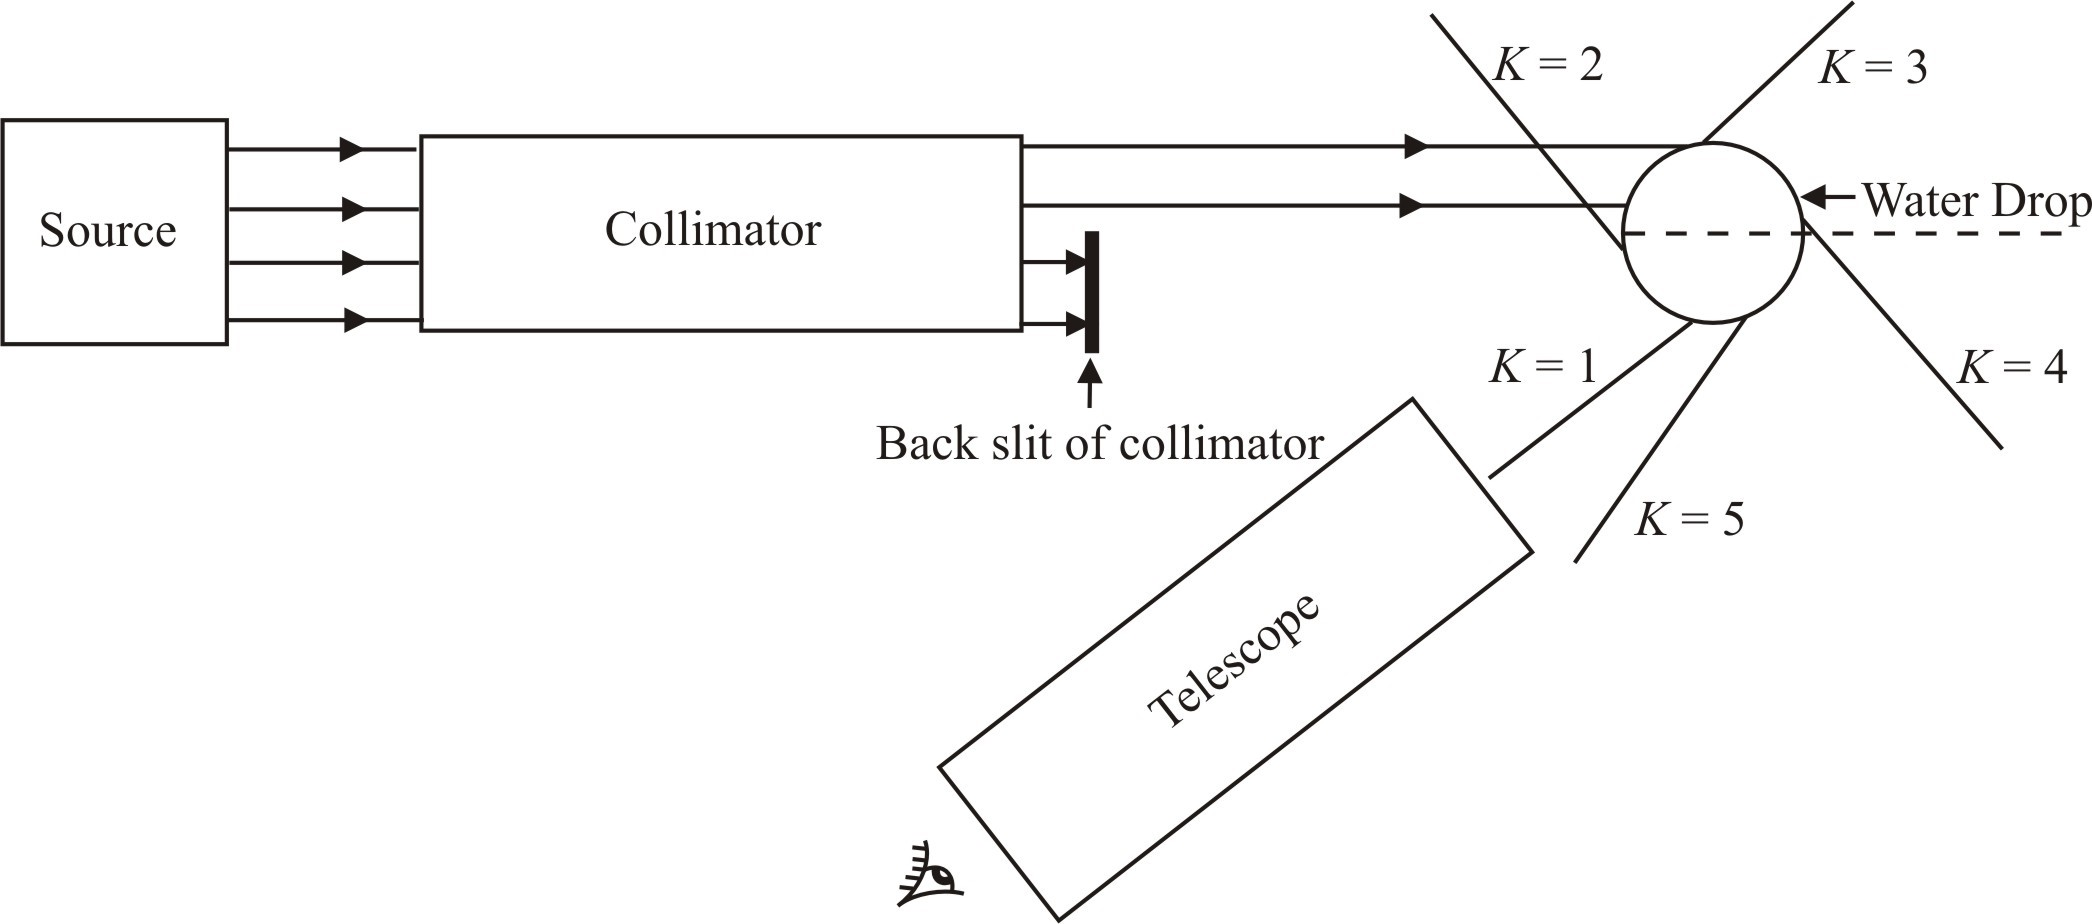
\includegraphics[width=0.70\textwidth]{figs/img2.jpg}
    \caption{Schematic of the experimental setup}
    \label{fig:experimentalsetup}
\end{figure}

\subsection*{Halogen lamp}

A high power (150 W, 24 V) tungsten filament halogen lamp (such as those commonly used in projectors) is provided as a source of white light. This lamp has a small filament, through which a high current (6 A) can be passed. It is mounted in a wooden box, on a stand whose height may be adjusted. The wooden box has four windows through which the light may be observed. A small fan is fixed inside the box to prevent excessive heating. The lamp has a specially designed 24 V (AC) power supply which powers it. The intensity of light emitted by the lamp may be changed on the supply. This is essential for observing the higher order rainbows, as one may need to have white light of higher intensity.

\subsection*{Miscellaneous}
A set of four small syringes, beakers, and Petri dishes are provided. Beakers may be used to store different liquids. Petri dishes can be placed on the prism table and are used to collect the liquid that falls from the syringe. Four different liquids (water, glycerine, clove oil, and an unknown liquid A) are also supplied. A magnifying reading torch is provided to read the circular scale, and a light blocking screen may be used to block the stray light falling on the drop. A spirit level may be used for levelling the prism table.

\subsection*{Useful Data}
\begin{itemize}
    \item Refractive index of water = 1.33
    \item Refractive index of glycerine = 1.47
    \item Refractive index of clove oil = 1.53
\end{itemize}

\subsection*{Warnings}
\begin{itemize}
\item Avoid observing the source directly through the telescope for long time.
\item Clamp the syringe on its holder carefully, so that it is held properly.
\item Use different Petri dishes, beakers, and syringes, for different liquids to avoid mixing.
\item Light reflected directly from the external surface of the drop will produce bright white glare spots that will hinder your observations. You will have to account for this and identify the rainbows carefully. 
\item The measurements have to be performed in a dark room.
\item Use only one window of the spectrometer for recording the readings. Use the same one throughout your experiment.
\end{itemize}


\section*{Experimental Problem}
\subsection*{Part A}

\begin{imp}
Begin by determining the least count of the spectrometer.
\end{imp}

Initially level the prism table using a spirit level. Fill the syringe with water and mount it on the holder clamped to the prism table. Keep the Petri dish on the prism table to collect the water drops, which may fall down from the nozzle of the syringe. Obtain a steady drop of water at the nozzle of the syringe. Adjust the height of the syringe such that the drop is seen at the centre of the field of view of the telescope.

Now adjust the alignment of the source, the collimator, the suspended drop, and the telescope, such that the drop is fully illuminated by the parallel beam of light. Partially close the back slit of the collimator so that only the vertical half of the water drop is illuminated by white light.

\begin{question}
\paragraph{Question:} If the light falling on the drop is parallel, does this mean that all the rays striking the drop will be refracted by the same angle? Explain your answer.
\end{question}

Keep the telescope, collimator, and the drop in the straight line; you will see white light coming from the central region of the drop. Note the angular position of the telescope at which this happens and treat it as the `direct' reading for further measurements. As stated earlier, this drop will produce rainbows of different orders, which can be observed at different angular positions around the drop. Thus the angular positions of different order rainbows (for water) will be as shown earlier in Figure (\ref{fig:firstorder1}). 

Observe the bright first-order rainbow to the right of the drop $(K = 1)$ first by eye and then by telescope. Adjust the telescope such that the bright red line of the spectrum can be seen. Measure the total angle of deviation $\phi_1$. Repeat the above step for the second order rainbow $(K = 2)$ and then for orders up to at least the fifth $(K = 5)$. (In this case you may make the intensity of lamp maximum.) Measure the total angle of deviation $\phi_K$ for different order rainbows. (Note: Before taking readings for each order, adjust the telescope to see the red light of the spectrum.) Plot a graph of $\phi_K (K = 1, 2, 3, \hdots)$ against $K$ for the different order rainbows formed due to a water drop.

\subsection*{Part B}
Replace the syringe and Petri dish containing water by the syringe and Petri dish containing glycerine and adjust the syringe to see the glycerine drop from all the positions of the telescope. Measure $\phi_2$ for glycerine. Repeat the above steps, for the clove oil and the given unknown liquid $A$. Determine $\phi_2$ for clove oil and the liquid $A$. Plot a graph of $\cos(\phi_2 / 6)$ against $1/\mu$ for water, glycerine and clove oil. 

\begin{question}
\paragraph{Question:} For $\mu = 1$ (air), what is the value of $\phi_2$? This should be taken as one of the points for plotting the above graph.
\end{question}
 

\subsection*{Part C}
Determine the value of $\mu$ for the liquid $A$ by measuring the deviation and extrapolating from the previous graph.



\section*{References}
\begin{enumerate}
\item Jearl D. Walker, \textit{Multiple rainbows from single drops of water and other liquids}, Am. J. Phys, 44 (5), 1976, pp. 421-433.
\item Kenneth Sassen, \textit{Angular scattering and rainbow formation in pendant drops}, J. Opt. Soc. Am., 69 (8), 1979, pp. 1083-1098. 
\item John Beynon, \textit{Introductory University Optics}, Prentice-Hall of India Pvt. Ltd., New Delhi, 1998, pp. 44-55.
\item Francis W. Sears, \textit{Optics}, Asian Publishing House (India), 1958, pp. 54-55. 

\end{enumerate}

